\documentclass[conference]{IEEEtran}
\IEEEoverridecommandlockouts

\usepackage{cite}
\usepackage{amsmath,amssymb,amsfonts}
\usepackage{graphicx}
\usepackage{textcomp}
\usepackage{xcolor}
\usepackage{booktabs}
\usepackage{url}
\usepackage{hyperref}

% Draft markers (remove before submission)
\newcommand{\todo}[1]{\textcolor{red}{[TODO: #1]}}

\begin{document}

\title{Client Monoculture in the Lightning Network:\\
Measured Concentration, an Observed Common-Mode Outage,\\ and Exposure-Aware Resilience}

\author{
\IEEEauthorblockN{\todo{author names}}
\IEEEauthorblockA{Bitcoin Data Labs\\
\todo{contact}}
}

\maketitle

% ==========================================================================================
\begin{abstract}
The Lightning Network is specified so that independent implementations interoperate, yet one of them,
LND, runs about 84\% of public nodes and holds about 85\% of public channel capacity. Prior work studied
resilience to random and degree-targeted node removal; how failures \emph{correlate with the software a node
runs} has not been measured. We combine 805 daily snapshots of public gossip (May~2023--October~2026), every
Lightning channel close and its follow-up spends from our own Bitcoin node (132,742 closes since January~2025),
and the funding transactions of all open channels (226,326). We (i)~infer each node's implementation from
announced feature bits and validate the rules against self-identifying aliases and an independent on-chain
signal, the wallet that builds a node's channel funding transactions (99.2\% held-out agreement);
(ii)~measure client concentration over three years; and (iii)~measure a real common-mode event: on
26~August~2026, during a wave of security fixes in every implementation, Core Lightning (CLN) maintainers asked
operators to take their nodes offline. The next day the share of channels toward CLN nodes that peers marked
disabled rose from 11.8\% to 38.1\% ($z=29$) while other clients stayed flat; 22\% of CLN nodes went dark,
concentrated among Tor-reachable operators, and a third of those were still dark five weeks later. Peers
force-closed channels with CLN nodes at 2.2 times their usual rate. Calibrating a failure model on this event,
we find that the outage stayed \emph{contained}: network-wide reachability fell by 7.8 percentage points,
at the edge of normal two-day churn (3.1--7.6), while reachability among CLN nodes fell by 24.5 points, 2--10
times more than in ordinary windows. The structural risk lies elsewhere. Minority clients reach each other
almost only through LND: 76--92\% of their channel capacity faces LND nodes, and without LND only 32\% of CLN,
42\% of Eclair and 11\% of LDK node pairs remain connected. Single hubs outweigh client cohorts: losing the 12
Eclair nodes, ACINQ above all, costs the surviving network more reachability than losing all 619 CLN nodes.
\end{abstract}

\begin{IEEEkeywords}
Lightning Network, Bitcoin, client diversity, common-mode failure, measurement, gossip, resilience
\end{IEEEkeywords}

% ==========================================================================================
\section{Introduction}
\label{sec:intro}

The Lightning Network (LN)~\cite{poon2016bitcoin} routes Bitcoin payments over a network of two-party payment
channels. Its protocol is defined by the BOLT specifications~\cite{bolt2,bolt3,bolt7,bolt9}, and four
independent implementations---LND, Core Lightning (CLN), Eclair and LDK---interoperate on the same public
network. Client diversity is often cited as a safety property: a bug in one implementation should not take
down the network. Whether it does in practice depends on two quantities that are rarely measured together:
\emph{who runs which software}, and \emph{how failures actually propagate} through the channel graph.

Topological studies of the LN~\cite{rohrer2019discharged,seres2020topological,lin2020lightning,martinazzi2020evolving}
measured centralization and resilience to random or degree-targeted node removal, and client
implementations have been inferred from gossip metadata~\cite{zabka2021node,espinasa2024decision}. Removing
``all LND nodes'' from a graph in which LND holds 85\% of capacity is trivially catastrophic and says little
about realistic failures, which are version-scoped, partial and temporary.

Between July and October 2026 every implementation shipped security fixes, for different
bugs~\cite{lndadvisories2026,clnadvisories2026,eclairldk2026}, and on 26~August CLN maintainers asked operators
to take nodes offline. This produced something rarely available: an observed, client-correlated outage in a
production payment network. We measure it and use it to calibrate a resilience model.

\paragraph*{Contributions}
\begin{itemize}
\item \textbf{C1: Validated client inference.} Feature-bit rules (with a keysend-based fix that keeps them valid
on historical snapshots) are checked against 795 self-identifying aliases and against an independent
on-chain signal, the wallet that builds a node's channel funding transactions. Agreement with the on-chain
signal is 99.2--99.3\% on held-out nodes (\S\ref{sec:inference}).
\item \textbf{C2: Three years of concentration.} From May~2023 to October~2026, LND's share of public node
capacity stayed between 85\% and 90\%; apparent changes in node shares coincide with a change in our gossip
vantage point and are mostly not real (\S\ref{sec:concentration}).
\item \textbf{C3: An observed common-mode outage.} We quantify the CLN shutdown: magnitude, who complied,
recovery, closing behaviour and cost, and separate it from confounds that look like incidents but are not
(\S\ref{sec:outage}).
\item \textbf{C4: Exposure-aware resilience.} Calibrated on C3 and compared with placebo windows and
targeted baselines, client-correlated failures stay contained; the structural risks are minority clients'
dependence on LND for connectivity and single-hub concentration (\S\ref{sec:resilience}).
\end{itemize}
All data are aggregated from public sources (gossip, the blockchain); code and aggregate datasets are released.

% ==========================================================================================
\section{Background and Related Work}
\label{sec:background}

\paragraph*{Gossip and channel state}
Nodes announce themselves (\texttt{node\_announcement}, including a feature-bit vector~\cite{bolt9}) and the
routing policy of each channel direction (\texttt{channel\_update})~\cite{bolt7}. A \texttt{channel\_update} can
mark its direction \emph{disabled}. A node that goes offline cannot announce anything; its \emph{peers} disable
their direction toward it. Outages are therefore visible as peer-side disabled flags, which is how we
measure them.

\paragraph*{Closing channels on-chain}
A channel is funded by a 2-of-2 output. A cooperative close spends it with a transaction both parties sign; a
unilateral (force) close broadcasts the latest commitment transaction, recognizable by its encoded commitment
number in \texttt{nLockTime} (upper byte \texttt{0x20}) and the input \texttt{nSequence} (upper byte
\texttt{0x80})~\cite{bolt3}. Its outputs are later swept (delayed \texttt{to\_local}, \texttt{to\_remote},
anchors, HTLCs) or, if a revoked state was published, claimed by the counterparty with a \emph{justice}
transaction.

\paragraph*{Resilience and attacks}
Rohrer et al.~\cite{rohrer2019discharged}, Seres et al.~\cite{seres2020topological}, Lin et
al.~\cite{lin2020lightning} and Martinazzi and Flori~\cite{martinazzi2020evolving} found the LN robust to random
failures and fragile to targeted hub removal. Attack studies exploit HTLC handling and congestion
\cite{harris2020flood,mizrahi2021congestion,perez2020lockdown}. None conditions failure on the implementation.

\paragraph*{Client inference}
Zabka et al.~\cite{zabka2021node} and Espinasa-Vilarrasa et al.~\cite{espinasa2024decision} infer implementations
from feature bits and policy defaults; we extend this with validation against an on-chain signal and with
rules that hold across three years of feature-set changes.

\paragraph*{Monoculture}
The risk of software monoculture is a classic argument in security~\cite{geer2003cyberinsecurity}, as is its
qualification: diversity helps only if failures are actually independent and the system does not route all
traffic through the dominant variant anyway~\cite{birman2009monoculture}. Our results quantify both sides for
the LN.

% ==========================================================================================
\section{Data and Vantage Point}
\label{sec:data}

\paragraph*{Daily gossip}
Since May~2023 our LND node has dumped its view of the public graph (\texttt{describegraph}) once a day. We
extract per-day node and channel-direction tables (features, addresses, policies, disabled flags). A quality
pass found 61 days on which the dump was an error response from LND (``wallet locked'' after restarts), 51
days of partial dumps (May--June~2024) and one stale day; these are excluded, leaving 805 days. The node was
replaced in mid-2024, which changed the view: before, about 42k channels and 8.4k nodes with channels; after,
41--50k channels and 11--13k nodes. We treat the two periods as \emph{vantage epochs} and compare levels only
within an epoch. Gossip is a single node's view of the public (announced) graph; unannounced channels, where
much LDK (wallets) and Eclair (Phoenix) usage lives, are not visible.

\paragraph*{On-chain closes and spends}
Our own Bitcoin Core node scans every block since January~2025 for spends of 257,570 known funding outputs.
For each close we record the transaction, block time and type (cooperative, force, splice); for each output of
a force close, the transaction that spends it and its type from the witness script. The data contain 132,742
closes (99,338 cooperative, 33,381 force, 23 splices) and 113,032 spends of force-close outputs. Batched
sweeps' fees are split across their inputs.

\paragraph*{Funding transactions}
For all 226,326 funding transactions of channels in our catalogue we record the funder wallet's construction
choices: \texttt{nVersion}, \texttt{nLockTime} policy, input \texttt{nSequence}, input and change script types,
output ordering, signature grinding, fee rate.

% ==========================================================================================
\section{Client Inference and Validation}
\label{sec:inference}

\paragraph*{Rules}
Implementation-specific feature bits decide most nodes: bits 2023 (script-enforced lease) or 31 (AMP) only
appear on LND; bit 37, or 29 together with 61, on Eclair; bit 11 together with 39 or 43 on CLN and Eclair, which
we separate by bit 55 (keysend, which CLN advertises by default---about 96\% of CLN-set nodes---and Eclair,
lacking native keysend, does not); bits
39/43/63 without 11 on LDK. Fallbacks (LND's default colour and alias, the modal CLTV default) yield low or
medium confidence. Operators with a publicly known implementation (ACINQ, Block) are attributed directly. An
earlier version without the keysend rule mislabeled ACINQ as CLN before 2025, when Eclair added bits 37 and 61;
rules must be validated against historical snapshots, not only the latest one.

\paragraph*{On-chain signal}
A funding transaction is built by the funder's wallet. On channels whose two endpoints share a
high-confidence label (so the funder's software is known), two wallet families separate cleanly: LND's
btcwallet (\texttt{nLockTime}~0, \texttt{nSequence}~\texttt{0x0}) and Core/BDK-style wallets (anti-fee-sniping
\texttt{nLockTime} at the current height, \texttt{nSequence}~\texttt{0xfffffffd}), used by CLN, Eclair (via
bitcoind) and BDK-based software. Since chain data does not reveal which endpoint funded a channel, we score
each node with a likelihood ratio in which a channel is funded by the node with probability $\theta=0.5$ and
otherwise by the peer, whose wallet distribution follows the peer's label; batch opens, where one node is
common to every channel funded by the transaction, identify the funder exactly. The signal measures the
\emph{wallet}, not the daemon: LND operators who fund channels from an external wallet look Core-style. It
cannot identify LDK or Eclair in general (our LDK sample is 99\% one operator).

\paragraph*{Validation}
Table~\ref{tab:classifier-eval} and Fig.~\ref{fig:validation} report two independent checks. Against 795 nodes
whose alias names their implementation (pooled over monthly snapshots; LND's default alias excluded because the
rules use it), precision and recall are 99.5\%/94\% for LND and 97\%/96\% for CLN; Eclair (9 nodes) and LDK (6)
are too few to say much. Most LND misses are nodes without announced features, which the rules leave Unknown.
Against the on-chain wallet family (5-fold held out for high-confidence labels), nodes labeled by LND-only bits
agree 99\% of the time ($n=3{,}199$), the CLN set with keysend 98\% ($n=471$); the CLTV-only fallbacks are
weakest (83--95\%) and account for five of the nine alias disagreements (e.g.\ LND nodes of one node-in-a-box platform
use CLTV~144, Eclair's default). A learned baseline ($k$-nearest neighbours on the feature-bit vector) does not
beat the rules on the same held-out folds (macro-F1 0.92 vs.\ 0.93). Over all nodes with at least five funding
transactions, held-out agreement between the on-chain family and high-confidence labels is 99.2--99.3\% and
98\% of nodes get a decision.

\begin{table}[t]
\centering
\caption{Validation of client inference (rules v3-2026-10-06). (a) 795 nodes whose
alias names their implementation (pooled over monthly snapshots, evaluated on the latest snapshot where they have a
channel); ``Unknown'' counts nodes the rules leave unlabeled (mostly no announced features). A learned baseline
($k$-NN, Jaccard, on the feature-bit vector) vs.\ rules on the same held-out folds: macro-F1 0.92 vs.\ 0.93 ($n=761$). (b) Share of nodes in each rule tier whose channel-funding wallet agrees with the
label (LND btcwallet for LND, Core/BDK-style otherwise), nodes with decisive on-chain evidence; high tiers graded with
held-out evidence.}
\label{tab:classifier-eval}
\small
\begin{tabular}{lrrrr}
\toprule
\multicolumn{5}{l}{(a) Alias anchors} \\
Client & $n$ & Precision (\%) & Recall (\%) & Unknown \\
\midrule
LND & 664 & 100 & 94 & 35 \\
CLN & 116 & 97 & 96 & 2 \\
Eclair & 9 & 62 & 56 & 3 \\
LDK & 6 & 100 & 100 & 0 \\
\bottomrule
\end{tabular}

\vspace{4pt}
\begin{tabular}{llrr}
\toprule
\multicolumn{4}{l}{(b) On-chain wallet family} \\
Label & Rule tier & $n$ & Agree (\%) \\
\midrule
CLN & CLN set + keysend & 471 & 98.1 \\
CLN & CLTV default only & 38 & 94.7 \\
CLN & CLTV default only (no features) & 18 & 83.3 \\
Eclair & Eclair bits (37, 29+61) & 10 & 90.0 \\
LDK & CLTV default only (no features) & 13 & 100.0 \\
LND & LND-only bits (2023/31) & 3,199 & 99.2 \\
\bottomrule
\end{tabular}
\end{table}


\begin{figure*}[t]
\centering
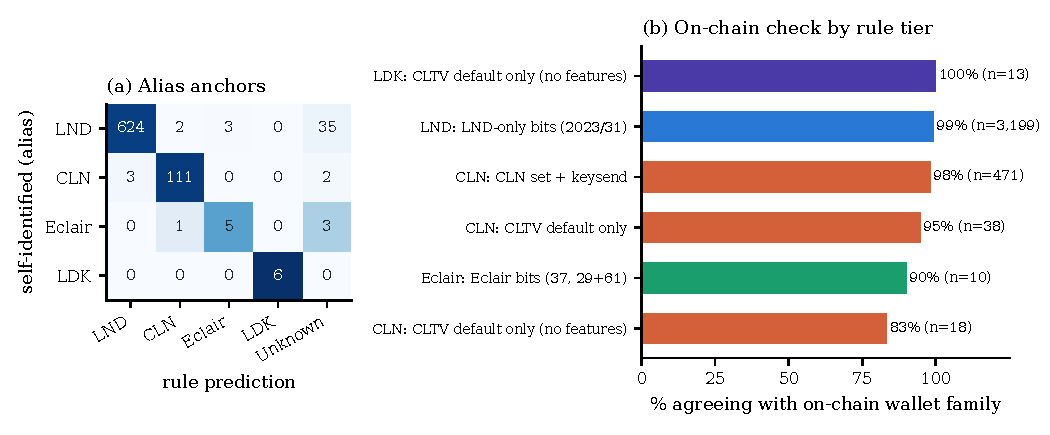
\includegraphics[width=\textwidth]{figures/fig2_classifier_validation.pdf}
\caption{Validation of client inference. (a) Nodes whose alias names their implementation vs.\ the rule
label. (b) Share of nodes in each rule tier whose channel-funding wallet agrees with the label (tiers with
$n\geq10$).}
\label{fig:validation}
\end{figure*}

% ==========================================================================================
\section{Concentration, 2023--2026}
\label{sec:concentration}

Figure~\ref{fig:share} shows monthly client shares of public nodes and of node capacity (each channel counted
for both endpoints). LND's share of capacity stayed between 85\% and 90\% throughout. Its share of nodes fell
from 91.8\% (May~2023) to 84.2\% (October~2026), but within each vantage epoch the change is about one point
(91.8\% to 90.9\%, and 85.1\% to 84.2\%); the step coincides with the change of our gossip node and the
appearance of many featureless (Unknown) nodes, not with a change in the network. The only clear within-epoch
trend is LDK's capacity share, from 1.7\% (July~2024) to 5.4\%, mostly Block's routing nodes. On the latest
snapshot (Table~\ref{tab:client-census}) LND runs 84.0\% of nodes (77.5\% counting only high-confidence labels)
and 84.4\% of capacity (84.3\%); CLN 8.5\% of nodes but 3.7\% of capacity; Eclair is a handful of nodes holding
6.1\% of capacity. Capital is more concentrated than node counts suggest for every minority client except
Eclair and LDK, whose capacity sits in very few operators.

\begin{figure*}[t]
\centering
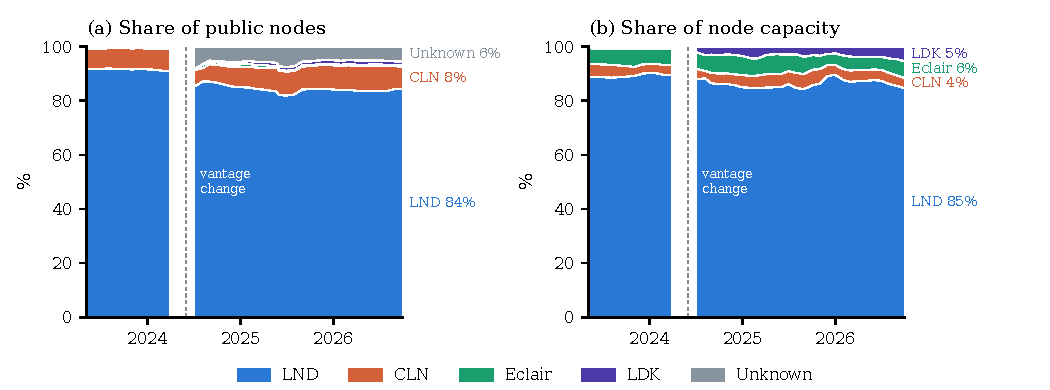
\includegraphics[width=\textwidth]{figures/fig1_client_share.pdf}
\caption{Client shares of public nodes with at least one channel (a) and of node capacity (b), first gossip
snapshot of each month. The dashed line marks the change of our gossip vantage point (mid-2024); months with
unusable dumps are omitted.}
\label{fig:share}
\end{figure*}

\begin{table}[htbp]
\caption{Empirical Distribution of Client Implementations Across the Public Lightning Network}
\label{tab:client_census}
\centering
\begin{tabular}{lrrrr}
\toprule
\textbf{Implementation} & \textbf{Nodes (\%)} & \textbf{Channels (\%)} & \textbf{Capacity (BTC)} & \textbf{Cap. Share (\%)} \\
\midrule
LND & -- & -- & -- & -- \\
Core Lightning (CLN) & -- & -- & -- & -- \\
Eclair & -- & -- & -- & -- \\
LDK & -- & -- & -- & -- \\
Unknown / Unclassified & -- & -- & -- & -- \\
\midrule
\textbf{Total Network} & 100.0\% & 100.0\% & -- & 100.0\% \\
\bottomrule
\end{tabular}
\end{table}


% ==========================================================================================
\section{The 2026 Security Wave and the Observed CLN Outage}
\label{sec:outage}

\paragraph*{Timeline}
In July CLN disclosed memory-exhaustion denial-of-service bugs. In early August, attackers read LND macaroons
from BTCPay Server instances older than 2.4.2 and force-closed merchant channels~\cite{btcpay2026}, an
application-layer credential leak rather than an LND protocol bug. On 11~August Lightning Labs published ten
LND advisories, four of high severity, all affecting old versions~\cite{lndadvisories2026}. On 26~August CLN
maintainers, facing a burst of vulnerability reports, asked operators to take nodes offline and stop
peering~\cite{clnadvisories2026}. Fixes followed in September for CLN, Eclair and LDK~\cite{eclairldk2026}, LND
published eight more advisories on 21~September, and on 2~October CLN warned of active exploitation of
versions up to 26.06.7. Every implementation was affected; the bugs were different.

\paragraph*{Measure}
For client $c$ and day $t$, $D_c(t)$ is the share of channel directions pointing \emph{toward} nodes of $c$ that
their peers mark disabled, unweighted and weighted by capacity. Client labels are fixed per node on
1~August~2026, so the incident cannot reshuffle cohorts. The baseline is 1--25~August.

\paragraph*{Magnitude}
On 27~August $D_{\mathrm{CLN}}$ rose from a baseline of $11.8\pm0.9\%$ to 38.1\% ($z=29$); by capacity from
7.4\% to 35.2\% (Table~\ref{tab:outage-effect}, Fig.~\ref{fig:outage}). LND, Eclair and LDK did not move
($|z|<2$). A difference-in-differences estimate against LND over the following two weeks, with a moving-block
bootstrap, gives $+14.2$ percentage points (95\% CI 11.2--16.0) by channel count and $+14.7$ (10.4--17.1) by
capacity. Removing, each day, the single node with the most disabled capacity leaves $+12.9$ (8.9--15.2), so
the capacity result is not one large node (Table~\ref{tab:outage-robustness}).

\begin{figure*}[t]
\centering
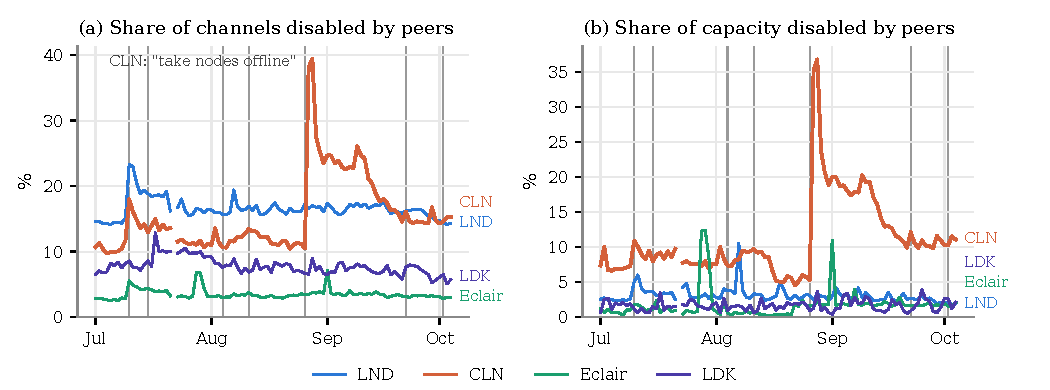
\includegraphics[width=\textwidth]{figures/fig3_observed_outage.pdf}
\caption{Share of channel directions toward each client's nodes that peers mark disabled, daily,
July--October~2026; by channel count (a) and by capacity (b). Vertical lines: incidents (\S\ref{sec:outage}).}
\label{fig:outage}
\end{figure*}

\begin{table}[t]
\centering
\caption{Share of channel directions toward each client cohort disabled by peers (\%). Baseline: daily mean $\pm$ sd, 2026-08-01 to 2026-08-25; peak: 2026-08-27; $z$ = (peak $-$ mean)/sd. Difference-in-differences, CLN vs.\ LND, 2026-08-27 to 2026-09-09 vs.\ baseline (95\% moving-block bootstrap CI, block 7 days): channels: +14.1 pp [+11.1, +16.0]; capacity: +13.6 pp [+9.3, +16.7].}
\label{tab:outage-effect}
\small
\begin{tabular}{lrrrrrr}
\toprule
 & \multicolumn{3}{c}{By channel count} & \multicolumn{3}{c}{By capacity} \\
\cmidrule(lr){2-4}\cmidrule(lr){5-7}
Client & Baseline & Peak & $z$ & Baseline & Peak & $z$ \\
\midrule
LND & 16.4 $\pm$ 0.8 & 16.6 & 0.3 & 3.5 $\pm$ 1.6 & 2.4 & -0.7 \\
CLN & 11.6 $\pm$ 0.9 & 37.5 & 29.3 & 6.4 $\pm$ 1.5 & 30.7 & 15.7 \\
Eclair & 3.3 $\pm$ 0.2 & 3.6 & 1.2 & 0.9 $\pm$ 0.7 & 1.9 & 1.5 \\
LDK & 7.7 $\pm$ 0.7 & 6.6 & -1.7 & 1.6 $\pm$ 0.6 & 1.3 & -0.6 \\
\bottomrule
\end{tabular}
\end{table}


\paragraph*{Who complied}
Of 624 CLN nodes not dark on 25~August, 137 (22\%) went dark---at least 80\% of the channels toward them
disabled, or absent from gossip---holding 33\% of CLN capacity. Larger operators complied more: 35\% of the
largest capacity quintile against 10--26\% of the others (Table~\ref{tab:outage-compliance}). The response split
by how nodes are reachable (Table~\ref{tab:outage-robustness}): among CLN nodes reachable over Tor only, the
disabled share rose from 13\% to 41\%, among dual-stack nodes from 5\% to 50\%, while among clearnet-only CLN
nodes it rose from 11\% to 19\% for two days and the two-week difference-in-differences is zero. Tor-only LND
nodes did not move (23.0\% to 23.4\%), so this was not a Tor outage. A plausible reading, which our data cannot
confirm, is that home and node-in-a-box operators, typically on Tor, followed the call, and hosted operators
did not.

\paragraph*{A transport-level contrast}
Gossip also shows a failure that was \emph{not} client-correlated: on 10~July~2026 the disabled share toward
Tor-only nodes of every client rose from 23\% to 43\% overnight (clearnet-only nodes flat) and decayed over two
weeks (Fig.~\ref{fig:tor}). Common-mode failures can follow transport as well as software.

\begin{figure}[t]
\centering
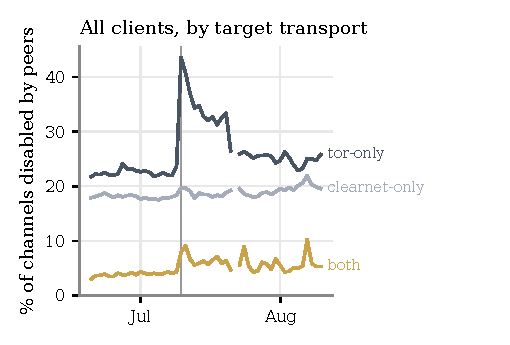
\includegraphics[width=\columnwidth]{figures/fig5_tor_event.pdf}
\caption{Disabled share toward Tor-only, clearnet-only and dual-stack nodes, all clients pooled. On
10~July~2026 Tor-only nodes of every client lost their peers at once.}
\label{fig:tor}
\end{figure}

\paragraph*{Recovery}
Of the 137 nodes, 39\% were back within three days and about half within a week; among nodes that returned,
the median time dark was three days (interquartile range 3--7). Twenty-two percent never reappeared, even for a day, by 4~October; counting nodes that came back and
went dark again, 32\% were dark on that date (Fig.~\ref{fig:recovery}). The 2~October exploitation warning produced no
comparable second wave ($D_{\mathrm{CLN}}$ 14.6\% on 2~October, 15.3\% on 4~October).

\begin{figure}[t]
\centering
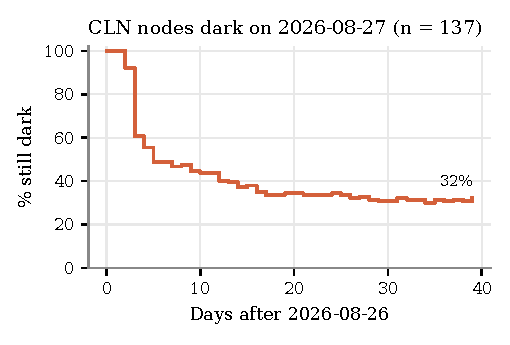
\includegraphics[width=\columnwidth]{figures/fig4_cln_recovery.pdf}
\caption{Share of the CLN nodes that went dark after the shutdown call that were still dark, by day.}
\label{fig:recovery}
\end{figure}

\paragraph*{Closing behaviour and confounds}
Read naively, closing data are full of ``incidents''. The two largest force-close days in the window were
single operators: on 3~August one LND node (NiceHash) was party to 226 force closes, and on 26~August---the day
of the CLN call---another LND node (Wallet of Satoshi) was party to 205. The early-August cooperative-close wave
was driven by large operators closing hundreds of channels each (Kraken alone was party to 12.6\% of closes on
2--16~August). We therefore separate \emph{mass-close events}, a node party to at least 20 force closes in a UTC
day (37 events since May, 30 by LND nodes), from organic force closes. Organic force closes of channels involving
a CLN node ran at 2.2 times their July--August rate during 26~August--8~September, 2.6 times relative to
channels between two LND nodes, whose rate fell slightly (0.83 times; Table~\ref{tab:outage-compliance}). Peers did
close on CLN nodes that went dark. Force closes are not a sign of theft: we find 17 justice spends in 21
months, the last on 11~July~2026; a successful theft leaves none, so this bounds attempts only from below.
The network shrank in August: of the 38,081 channels in gossip on 1~August, 14,547 were gone by 4~October and
97\% of those closed on-chain (10,464 in August), against 6,833 new channels.

\paragraph*{Cost}
The median force close cost 1,223~sat in fees including the sweeps of its outputs, six times a cooperative close
(209~sat); all 8,847 force closes since May paid 0.17~BTC in total. The on-chain cost of the episode was
negligible; its cost was liquidity locked behind time-locks and channels lost.

\begin{table}[t]
\centering
\caption{(a) CLN nodes that went dark after the shutdown call (not dark on 2026-08-25, dark on 2026-08-28), by
pre-incident node capacity quintile. (b) Organic force closes per 1{,}000 open public channels per day involving
each cohort, 2026-07-01--08-25 (baseline) vs.\ 2026-08-26--09-08 (window); mass-close events (one node in
$\geq 20$ force closes in a UTC day) excluded.}
\label{tab:outage-compliance}
\small
\begin{tabular}{lrrr}
\toprule
\multicolumn{4}{l}{(a) Compliance by size} \\
Quintile & Capacity (BTC) & Nodes & Went dark (\%) \\
\midrule
Q1 & 0.000--0.004 & 125 & 25.6 \\
Q2 & 0.004--0.010 & 125 & 10.4 \\
Q3 & 0.010--0.042 & 125 & 25.6 \\
Q4 & 0.043--0.208 & 125 & 31.2 \\
Q5 & 0.210--44.488 & 125 & 35.2 \\
\midrule
\multicolumn{4}{l}{(b) Organic force-close rate} \\
\end{tabular}
\begin{tabular}{lrrrr}
Cohort & Baseline & Window & Ratio & vs.\ LND$\leftrightarrow$LND \\
\midrule
CLN & 1.38 & 3.02 & 2.18 & 2.64 \\
Eclair & 0.80 & 0.83 & 1.04 & 1.26 \\
LDK & 14.17 & 8.45 & 0.60 & 0.72 \\
LND$\leftrightarrow$LND & 1.02 & 0.84 & 0.83 & 1.00 \\
\bottomrule
\end{tabular}
\end{table}

\begin{table}[t]
\centering
\caption{Robustness of the CLN outage effect. Baseline and peak as in Table~\ref{tab:outage-effect};
DiD vs.\ LND targets in the same subset, 95\% moving-block bootstrap CI. Target transport from node
announcements on 20260801.}
\label{tab:outage-robustness}
\small
\begin{tabular}{lrrrr}
\toprule
Variant & Baseline (\%) & Peak (\%) & $z$ & DiD (pp) \
\midrule
All targets, by channels & 11.6 & 37.5 & 29.3 & +14.1 [+11.1, +16.0] \\
All targets, by capacity & 6.4 & 30.7 & 15.7 & +13.6 [+9.3, +16.7] \\
By capacity, largest node removed & 5.3 & 27.6 & 20.8 & +11.5 [+7.8, +13.9] \\
Clearnet-only targets, by channels & 9.2 & 17.9 & 9.3 & +0.3 [-1.2, +2.3] \\
Tor-only targets, by channels & 15.7 & 39.0 & 9.4 & +23.1 [+20.8, +25.2] \\
Both targets, by channels & 6.9 & 47.4 & 39.6 & +16.1 [+10.0, +18.7] \\
\bottomrule
\end{tabular}
\end{table}


% ==========================================================================================
\section{Exposure-Aware Resilience}
\label{sec:resilience}

\paragraph*{Model}
We take the routable core of the public graph on 25~August~2026, the day before the call: channels whose two
directions are announced and enabled (73\% of announced channels; 4,435 nodes). A payment of $a$ satoshis can use
a channel whose capacity is at least $a$ (optimistic) or $2a$ (balances split evenly). Failures are modelled as
\emph{exposure}, a fraction $p$ of a client's nodes being unavailable, not deletion of the client. Our main
measure is $R_{\mathrm{all}}(a)$, the share of the pre-failure node pairs still connected by a path of usable
channels, so pairs involving a failed node count as lost; we also report $R(a)$ among surviving nodes and
$R_c(a)$ among pairs of client $c$. Connectivity is an upper bound on what routing achieves (no fees, no
in-flight HTLCs, no liquidity uncertainty beyond the threshold). Random scenarios average 50 draws.

\paragraph*{Calibration and placebo}
The observed footprint is the set of nodes of the 25~August core with no usable channel left on 27~August (383
nodes, 105 of them CLN). It reduced $R_{\mathrm{all}}$ for 100k-sat payments by 7.8 points. Two-day windows
earlier in August, with no incident, reduced it by 3.1--7.6 points: the network-wide footprint is at the edge of
normal churn. For pairs of CLN nodes the loss was 24.5 points, against 2.3--10.6 in the placebo windows.

\paragraph*{Scenarios}
Table~\ref{tab:scenarios} and Fig.~\ref{fig:curves} compare failures. The calibrated scenario ($\hat p=0.22$ of
CLN nodes failing at random, 136 nodes) leaves $R$ among survivors at 78.8\%, against 77.9\% when the same number
of nodes fails at random across all clients: for the rest of the network, a CLN-wide outage behaves like random
failure, because CLN nodes are mostly peripheral. The damage stays inside the cohort ($R_{\mathrm{CLN}}$ falls to
46\%). Removing the same number of nodes chosen by degree leaves 27.6\%, by capacity 33.7\%. Losing all 619 CLN
nodes leaves survivors at 76.2\%; losing the 12 Eclair nodes, which hold 5.8\% of capacity and are dominated by
ACINQ, leaves 63.9\%. Single hubs matter more than client cohorts. Per unit of failed capacity, failures confined
to Eclair are the most damaging and failures confined to LDK the least (Fig.~\ref{fig:curves}).

\paragraph*{Dependence on LND}
Minority clients' channel capacity faces LND: 76\% for CLN, 92\% for Eclair and 81\% for LDK
(Fig.~\ref{fig:matrix}); CLN keeps 15\% of its capacity among CLN peers. Without LND nodes, only 32\% of CLN pairs,
42\% of Eclair pairs and 11\% of LDK pairs remain connected for 100k-sat payments (14\%, 42\% and 9\% for 1M sats).
Minority clients do not form a network of their own; their diversity does not translate into independent
reachability.

\begin{table*}[t]
\centering
\caption{Failure scenarios on the 2026-08-25 public graph (channels enabled in both
directions), payment size 100,000 sats, optimistic liquidity. $R_{\mathrm{all}}$: \% of pre-failure node pairs still connected (pairs with a failed
node count as lost); $R$: \% of online node pairs connected by a path of
channels that can carry the payment; $R_c$: same as $R$, for pairs of surviving nodes of client $c$; LCC cap.: \% of usable capacity in the largest
component. Random scenarios: mean of the Monte Carlo runs.}
\label{tab:scenarios}
\small
\begin{tabular}{lrrrrrrrr}
\toprule
Scenario & Failed & Cap.\ (\%) & $R_{\mathrm{all}}$ & $R$ & $R_{\mathrm{CLN}}$ & $R_{\mathrm{Eclair}}$ & $R_{\mathrm{LDK}}$ & LCC cap. \\
\midrule
Intact & 0 & 0.0 & 79.8 & 79.8 & 79.2 & 83.3 & 80.0 & 100.0 \\
Observed: lost all usable channels, Aug 27 & 383 & 0.5 & 72.0 & 86.3 & 79.4 & 83.3 & 81.5 & 99.0 \\
  of which CLN nodes only & 105 & 0.2 & 76.0 & 79.8 & 79.4 & 83.3 & 80.0 & 99.6 \\
Calibrated CLN ($\hat p$ = 0.22) & 136 & 0.9 & 74.1 & 78.8 & 76.3 & 83.3 & 79.1 & 98.2 \\
Same count, random nodes & 136 & 3.1 & 73.2 & 77.9 & 76.8 & 82.5 & 77.6 & 93.9 \\
Same count, top degree & 136 & 70.5 & 25.9 & 27.6 & 24.8 & 33.3 & 14.7 & 8.9 \\
Same count, top capacity & 136 & 80.2 & 31.7 & 33.7 & 30.1 & 21.4 & 10.4 & 6.6 \\
All LND nodes fail & 3,704 & 85.4 & 0.8 & 28.3 & 31.8 & 42.4 & 11.1 & 2.3 \\
All CLN nodes fail & 619 & 3.9 & 56.4 & 76.2 & -- & 83.3 & 76.2 & 92.8 \\
All Eclair nodes fail & 12 & 5.8 & 63.5 & 63.9 & 59.1 & -- & 69.0 & 88.4 \\
All LDK nodes fail & 95 & 4.8 & 76.2 & 79.6 & 78.9 & 83.3 & -- & 91.1 \\
\bottomrule
\end{tabular}
\end{table*}


\begin{figure*}[t]
\centering
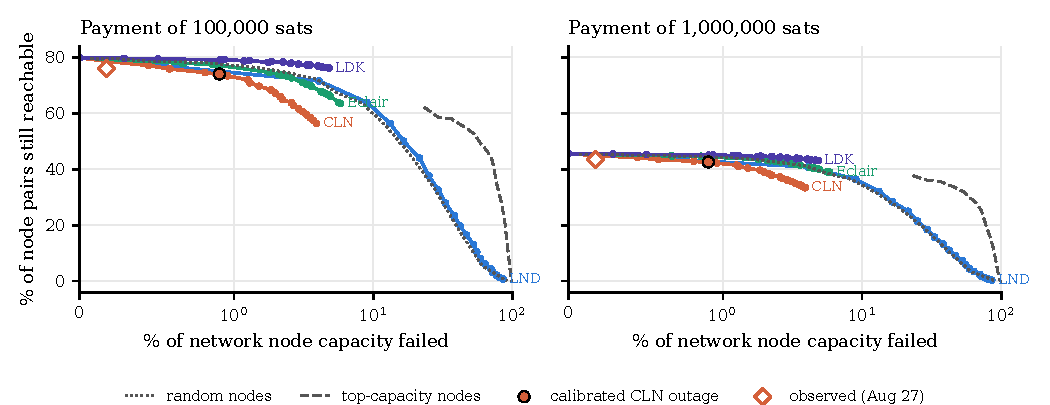
\includegraphics[width=\textwidth]{figures/fig6_resilience_curves.pdf}
\caption{Share of node pairs still reachable vs.\ share of network node capacity failed, for random failures
within each client (lines with markers), random failures across all nodes (dotted) and the largest nodes by
capacity (dashed). Dot: calibrated CLN outage; diamond: observed footprint of 27~August (CLN nodes). Routable core
of 25~August~2026; left: 100k sat, right: 1M sat payments.}
\label{fig:curves}
\end{figure*}

\begin{figure}[t]
\centering
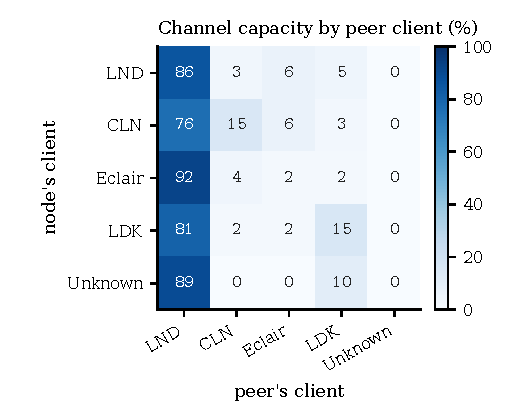
\includegraphics[width=\columnwidth]{figures/fig7_client_capacity_matrix.pdf}
\caption{Share of each client's channel capacity (rows) by the client of the peer (columns), routable core of
25~August~2026.}
\label{fig:matrix}
\end{figure}

% ==========================================================================================
\section{Discussion}
\label{sec:discussion}

\paragraph*{Containment, not collapse}
The first measured client-wide outage in the LN was absorbed: the network as a whole lost about as much
reachability as in an ordinary two days, while the affected cohort lost a quarter of its internal
reachability and saw peers force-close at twice the usual rate. Client-correlated failure was costly for the
client's own users, not for everyone else, because the affected nodes were peripheral.

\paragraph*{Where the risk is}
Two structural findings matter more than the share numbers. First, minority clients reach each other through LND;
a failure of LND (or of the LND nodes that act as hubs) would isolate them from each other, not only from LND
users. Diversity that routes through the dominant client provides less independence than node counts suggest.
Second, a handful of hubs, regardless of client, carry the network; ACINQ alone outweighs the entire CLN cohort for
the survivors' reachability. Hub diversity---which software the largest routing nodes run---is the quantity to
watch.

\paragraph*{Operational lessons}
Compliance with an emergency call was voluntary and uneven (22\% of CLN nodes, concentrated among Tor-reachable
operators); a third of those were still dark after five weeks, so emergency shutdowns have lasting costs for
operators who follow them. Large single-operator events (mass closes, a custodial wallet closing hundreds of
channels the day of the CLN call) are easily mistaken for network-wide effects; concentration checks belong in
any incident analysis. For the measurement community: gossip pipelines should validate dumps (we found 61 days of
saved error responses) and record their vantage point.

\paragraph*{Recommendations}
(i)~Monitor peer-side disabled shares per client and per transport as an early-warning signal; it is cheap and
was unambiguous here. (ii)~Encourage channels between minority-client hubs, so that CLN, Eclair and LDK users
are not connected only through LND. (iii)~Track the implementation of the largest hubs, not only node shares.
(iv)~Coordinate emergency guidance so that ``go offline'' is scoped by version and duration.

% ==========================================================================================
\section{Limitations}
\label{sec:limitations}
Our gossip is one node's view of the announced graph, which changed in mid-2024; unannounced channels (most
LDK and Phoenix usage) are invisible. Feature-bit rules can be wrong for new releases and are weak where nodes
announce no features; the on-chain signal identifies wallets, not daemons, and cannot separate CLN from Eclair
or identify LDK. Disabled flags record peers' views with some delay and cannot distinguish a node that is
offline from one that refuses peers. The resilience model measures connectivity under capacity thresholds, an
upper bound on payment success; we do not model fees, liquidity distribution, HTLC limits or private routing
hints. Chain data do not reveal which side broadcast a force close. Some incident dates are approximate. We did
not analyse routing-policy defaults (planned: \S\ref{sec:conclusion}).

\section{Ethics}
We use only public gossip and blockchain data and report aggregates. We name large public operators only for
their closing behaviour, which is public on-chain, and publish no lists of potentially vulnerable nodes.

% ==========================================================================================
\section{Conclusion}
\label{sec:conclusion}
LND holds about 85\% of public Lightning capacity, a share that has barely moved in three years. When an
emergency took a fifth of CLN nodes offline in August~2026, the network absorbed it: the damage stayed within
the CLN cohort. The fragility lies in the structure that diversity statistics hide: minority clients connect
through LND, and a few hubs carry the network. Future work: simulate client-specific pathfinding~\cite{pickhardt2021optimally} to test whether
policy defaults bias route selection, validate reachability with probing, and extend the on-chain fingerprint to
identify funders exactly by linking change outputs.

\section*{Data and Code Availability}
\todo{repository URL}. Scripts reproduce every figure and table from the data lake; aggregate datasets are
released with the paper.

\bibliographystyle{IEEEtran}
\bibliography{references}

\end{document}
